\documentclass{article}

% Packages
\usepackage[utf8]{inputenc} % UTF-8 input encoding
\usepackage[T1]{fontenc} % Font encoding
\usepackage{amsmath, amssymb} % Math packages
\usepackage{enumitem} % For customizing lists
\usepackage{lipsum} % For generating dummy text
\usepackage{listings}
\usepackage{graphicx}


\lstset{%
  language=bash,
  basicstyle=\fontfamily{pcr}\selectfont,
  commentstyle=\bfseries,
  escapeinside={(*@}{@*)}
}

\newcommand{\comment}[1]{\# here is a comment: #1}
\newcommand\floor[1]{\lfloor#1\rfloor}
\newcommand\ceil[1]{\lceil#1\rceil}

% Title and author information
\title{Algorithms (6470) HW01}
\author{Alex Darwiche}
\date{\today}

\begin{document}

\maketitle

\section*{Answers}

% Question 1
\subsection*{Q1}
\begin{enumerate}[label=(\alph*)]
    \item Psuedocode for finding frequency of a number in a given array A:
    \begin{lstlisting}[frame=single]
    def count(Array A):
        counter = 0
        value = someNumber
        for i = 1 to A.Length:
            if A[i] == value:
                counter = counter + 1
        return counter

    \end{lstlisting}
    \subsection*{Use Loop Invariant Technique}
    \item Initalization ("Loop Start"): i = 1
    \subitem (1) Calling count on A gives the freq of value: counter = count(A[1...i])
    \subitem (2) When i = 1, counter = count(A[1...1]) = count(A[1])
    \subitem (3) count(A[1]) returns 1 if A[1] == value and 0 otherwise.
    \subitem (4) True prior to first iteration. \textbf{Intialization checked.}

    \item Maintenance: step = i
    \subitem (1) Assume "counter for i-1" = count(A[1...i-1])
    \subitem (2) For step i, counter = count(A[1...i-1], A[i]) = count(A[1...i])
    \subitem (3) True at step i, given step i-1. \textbf{Maintenance checked.}

    \item Termination ("Loop End"): i = n+1
    \subitem (1) Assume "counter for i-1" = count(A[1...i-1])
    \subitem (2) For step n+1, counter = count(A[1...n+1-1]) = count(A[1...n])
    \subitem (3) True at step n+1. \textbf{Termination checked.}
\end{enumerate}

% Question 2
\subsection*{Q2}
\begin{enumerate}[label=(\alph*)]
    \item Prove: $\floor{an}$ + $\ceil{(1-a)*n}$ = n.
    \subitem (1) $\ceil{(1-a)*n}$ = $\ceil{n-an}$
    \subitem (2) $\ceil{n-an}$ = n + $\ceil{-an}$
    \subitem (3) $\ceil{-an}$ = - $\floor{an}$, so n + $\ceil{-an}$ = n - $\floor{an}$
    \subitem (4) Sub above back into original equation: $\floor{an}$ + n - $\floor{an}$ = n.
    \subitem (5) The $\floor{an}$ terms cancel out, and: n = n. \textbf{Proof complete.}
\end{enumerate}

% Question 3
\subsection*{Q3}
\begin{enumerate}[label=(\alph*)]
    \item Given $f(n) \in O(g(n))$, show $g(n) \in \Omega(f(n))$
    \subitem (1) Assumption: $f(n) \leq c*g(n)$
    \subitem (2) Prove: $g(n) \geq k*f(n)$
    \subitem (3) $f(n) \leq c*g(n)$ is equivalent to $\frac{1}{c} * f(n) \leq g(n)$
    \subitem (4) $\frac{1}{c} * f(n) \leq g(n)$ can be flipped: $g(n) \geq \frac{1}{c} * f(n)$
    \subitem (5) So, we've now got the form of Big Theta: $g(n) \geq \frac{1}{c} * f(n)$
    \subitem (6) If we assume: $\frac{1}{c} = k$, then $g(n) \geq k * f(n)$ and $g(n) \in \Omega(f(n))$.
    \subitem (7) So, if $k = 1$, then $g(n) \in \Omega(f(n))$ for $n \geq 1$ .
    \subitem (8) This follows from the transpose symmetry in the textbook. \textbf{Proof complete.}.
    
    \item Given $p(n) \in O(f(n))$ then $p(n)f(n) \not\in O(f(n))$
    \subitem (1) Assumption: $p(n) \leq c*f(n)$
    \subitem (2) Prove this is not possible: $p(n)f(n) \leq c * f(n)$
    \subitem (3) Multiply each side of the assumption by f(n): $f(n) * p(n) \leq c * f(n)^2$ 
    \subitem (4) So, this leaves 1. $f(n) * p(n) \leq c * f(n)^2$ and 2. $p(n)f(n) \leq c * f(n)$
    \subitem (5) I believe that given $p(n) \leq c*f(n)$, we can now see that $p(n)f(n) \in O(f(n)^2)$ and $p(n)f(n) \not\in O(f(n))$
    \subitem (6) I think those 2 expressions are contradictory, just proving the original statement. \textbf{Proof complete.}.

    \item Show: $max(f(n), g(n)) \in O(f(n)+g(n))$
    \subitem The max of 2 functions will return either function 1 or function 2. So we need to check the math for the case where f(n) > g(n) and the case where g(n) > f(n).
    \subitem (1) Assumption: $max(f(n), g(n))$ = $f(n)$ or $g(n)$
    \subitem (2) Prove: $max(f(n), g(n)) \leq c * [f(n)+g(n)]$
    \subitem (3) $c * [f(n)+g(n)]$  = $c*f(n)+c*g(n)$
 
    \subitem (4) Prove Case 1: $f(n) \leq c * [f(n)+g(n)]$
    \subitem (5) So, $f(n) \leq c*f(n)+c*g(n)$ rearrange: $f(n) * \frac{(1-c)}{c} \leq g(n)$
    \subitem (6) $f(n)$ and $g(n)$ are non negative, when $c \geq 1$, this inequality will be true for all n>0: $f(n) * \frac{(1-c)}{c} \leq g(n)$
    \subitem (7) \textbf{So for Case 1: Proof complete.} 

    \subitem (8) Prove Case 2: $g(n) \leq c * [f(n)+g(n)]$
    \subitem (9) So, $g(n) \leq c*f(n)+c*g(n)$ rearrange: $g(n) * \frac{(1-c)}{c} \leq f(n)$
    \subitem (10) $f(n)$ and $g(n)$ are non negative, when $c \geq 1$, this inequality will be true for all n>0: $g(n) * \frac{(1-c)}{c} \leq f(n)$
    \subitem (11) \textbf{So for Case 2: Proof complete.} 

    \item Show: $n! \in O(n^n)$
    \subitem (1) n! = n*(n-1)*(n-2)*...*(1)
    \subitem (2) $n^n$ = n*n*n*n*n*...*n
    \subitem (3) So, $n! \leq c * n^n$ for c = 1 and $n \geq 1$.
    \subitem (4) $n*(n-1)*...*(1) \leq c * n*n*...*n$
    \subitem (5) Given $n^n$ is greater at each step after n=1, $n! \in O(n^n)$
    \textbf{Proof complete.} 


\end{enumerate}

% Question 4
\subsection*{Q4}
\begin{enumerate}[label=(\alph*)]
    \item Prove: $f(n) = 4n^2 - 50n + 10 \in o(n^3)$
    \subitem (1) Need to show that $\lim_{n\to\infty} \frac{f(n)}{n^3} = 0$
    \subitem (2) Break up the limit into 3 parts.
    \subitem (3) Part 1: $\lim_{n\to\infty} \frac{4n^2}{n^3}$ = $\lim_{n\to\infty} \frac{4}{n} = 0$
    \subitem (4) Part 2: $\lim_{n\to\infty} \frac{50n}{n^3}$ = $\lim_{n\to\infty} \frac{50}{n^2} = 0$
    \subitem (5) Part 3: $\lim_{n\to\infty} \frac{10}{n^3} = 0$
    \subitem (6) So, $\lim_{n\to\infty} \frac{4n^2}{n^3}$ + $\lim_{n\to\infty} \frac{50n}{n^3}$ + $\lim_{n\to\infty} \frac{10}{n^3} = 0$
    \subitem (7) Since this limit goes to zero, $f(n) = 4n^2 - 50n + 10 \in o(n^3)$

    \item Prove: $f(n) = n^3 - 5n^2 - 5 \in \omega(n^2)$
    \subitem (1) Need to show that $\lim_{n\to\infty} \frac{f(n)}{n^2} = \infty$
    \subitem (2) Break up the limit into 3 parts.
    \subitem (3) Part 1: $\lim_{n\to\infty} \frac{n^3}{n^2}$ = $\lim_{n\to\infty} n = \infty$
    \subitem (4) Part 2: $\lim_{n\to\infty} \frac{5n^2}{n^2}$ = $\lim_{n\to\infty} 5 = 5$
    \subitem (5) Part 3: $\lim_{n\to\infty} \frac{-5}{n^2} = 0$
    \subitem (6) So, $\lim_{n\to\infty} \frac{f(n)}{n^2} = \infty + 5 + 0 = \infty$
    \subitem (7) Since this limit goes to $\infty$, $f(n) = n^3 - 5n^2 - 5 \in \omega(n^2)$

\end{enumerate}

% Question 5
\subsection*{Q5}
\begin{enumerate}[label=(\alph*)]
    \item Substitution Method: $T(n) = T(n/2) + n^3$
    \subitem (1) a = 1, b = 2, d = 3. This means we use Master's Theorem Guess of $O(n^3)$ because $a < b^d = 1 < 2^3$
    \subitem (2) $T(n) \leq cn^3$
    \subitem (3) $T(n/2) \leq c* (\frac{n}{2})^3$
    \subitem (4) $T(n) = c*(\frac{n}{2})^3 + n^3$ = $n^3 + \frac{c*n^3}{8}$
    \subitem (5) We now need to get to the form: $T(n) = cn^3 - (something)$
    \subitem (6) $\frac{c*n^3}{8} = cn^3 - \frac{7c*n^3}{8}$
    \subitem (7) $n^3 + \frac{c*n^3}{8}$ = $cn^3 + n^3 - \frac{7c*n^3}{8}$
    \subitem (8) $cn^3 + n^3 - \frac{7c*n^3}{8}$ = $cn^3 + n^3 * (1 - \frac{7c}{8})$ = $cn^3 - n^3 * (\frac{7c}{8} - 1)$
    \subitem (9) So, finally: something = $(\frac{7c}{8} - 1) > 0$
    \subitem (10) Solve for c and get: $c > \frac{8}{7}$, for n > 0

    \item Substitution Method: $T(n) = 3T(n/3) + n$
    \subitem (1) a = 3, b = 3, d = 1. This means we use Master's Theorem Guess of $O(nlogn)$ because $a = b^d = 3 = 3^1$
    \subitem (2) $T(n) \leq c*n*logn$
    \subitem (3) Show that $T(n) = c*n*logn - (something)$
    \subitem (4) $T(n/3) \leq c*\frac{n}{3}log\frac{n}{3}$
    \subitem (5) $T(n) = 3 * (c\frac{n}{3}log\frac{n}{3}) + n$ = $cn*(logn-log3) + n$
    \subitem (6) $T(n) = cnlogn + n -cnlog3$ = $cnlogn - n (clog3 - 1)$
    \subitem (7) Show that, something: $(clog3 - 1) > 0$ = $c = \frac{1}{log3}$, for n > 2

    \item Substitution Method: $T(n) = 3T(n-1) + 1$
    \subitem (1) a = 3, b = 1, d = 0. This means we use Master's Theorem Guess of $O(3^n)$ because $a > b^d = 3 > 3^0$
    \subitem (2) $T(n) \leq c*3^n$
    \subitem (3) Show that $T(n) = c*3^n - (something)$
    \subitem (4) $T(n-1) \leq c*3^{n-1}$
    \subitem (5) $T(n) =  3*c*3^{n-1} + 1$ = $c3^n+1$
    \subitem (6) So, we've reached a point where we need to make a new guess given we cannot make this into the form: $c*3^n - (something)$. We look at our last step and use that as our new guess, given its $c3^n - lowerOrderTerms$
    \subitem (7) New Guess: $T(n) \leq c*3^n - 1$
    \subitem (8) $T(n) =  3*(c*3^{n-1}-1)+ 1$ = $c3^n - 3 + 1$ = $c3^n - 2$
    \subitem (9) $T(n) = c3^n - 2$ for c>1 and n>1.
 

\end{enumerate}

% Question 6
\subsection*{Q6}
\begin{enumerate}[label=(\alph*)]
    \item Show Substitution Method Failure and Lower Order Reguess: $T(n) = 8T(n/2) + n^2$
    \subitem (1) Trying to show that $T(n) \leq cn^3$ fails but $T(n) \in O(n^3)$
    \subitem (2) $T(n) \leq cn^3$
    \subitem (3) $T(n/2) \leq \frac{cn^3}{8}$
    \subitem (4) $T(n) = 8*\frac{cn^3}{8} + n^2$ = $cn^3 + n^2$
    \subitem (5) There is no way to make $n^2 < 0$ so, we need to reguess.
    \subitem (6) Reguess: $T(n) \leq cn^3 - kn^2$
    \subitem (7) $T(n/2) \leq \frac{cn^3}{8} - \frac{kn^2}{4}$
    \subitem (8) $T(n) = 8*\frac{cn^3}{8} - 8*\frac{kn^2}{4} + n^2$ = $cn^3 - 4kn^2 + n^2$ = $cn^3 - n^2(4k - 1)$
    \subitem (9) So, now $(4k-1) > 0$ or $k > \frac{1}{4}$ and n>1.
    

    
    
\end{enumerate}

% Question 7
\subsection*{Q7}
\begin{enumerate}[label=(\alph*)]
    \item The following shows how you'd use a recurrence tree to gather the information needed to solve the recurrence relationship for $T(n) = 2T(n/2) + n^3$
    \subitem 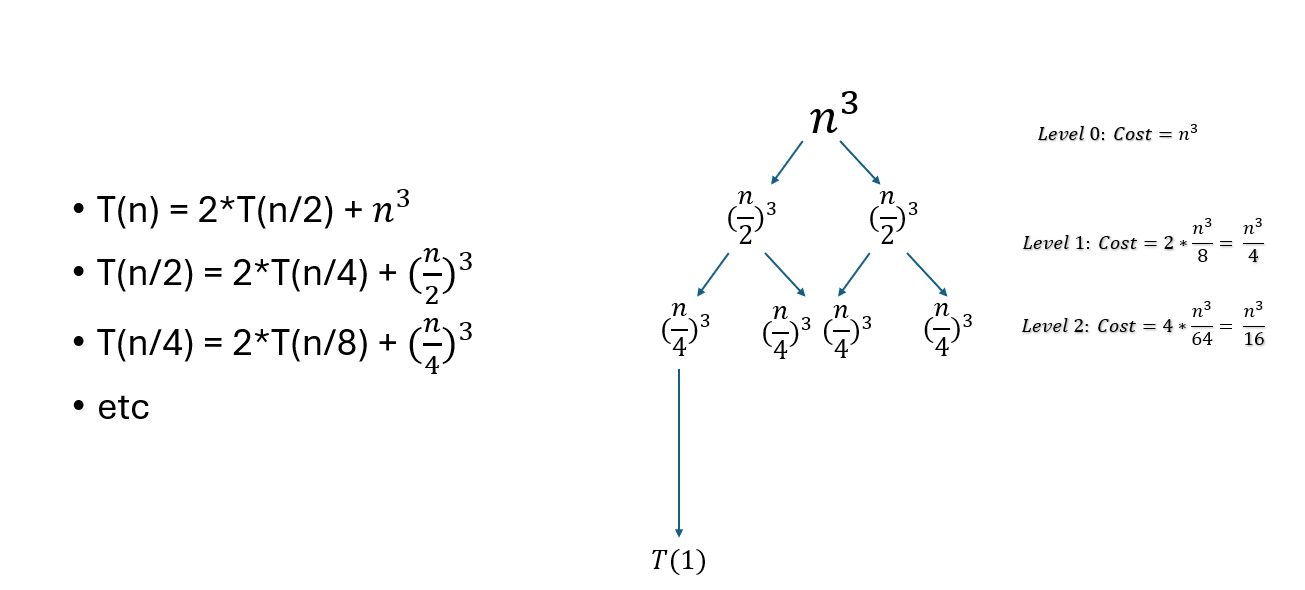
\includegraphics[width=1\textwidth]{tree.png}
    \item Now we can express the number of levels "i" by solving $\frac{n}{4^i} = 1$ and $i = log_{4}n$
    \item Next, we need to determine the cost at each level. Given the tree, it appears to be a geometic series where a = 1 and r = 1/4.
    \item $\sum\limits_{i = 0}^{logn} {n^3 * \frac{1}{4^i}} = n^3 * \sum\limits_{i = 0}^{logn} {\frac{1}{4^i}} = n^3 * \frac{1}{{1 - 1/4}}$ = $\frac{4n^3}{3}$
    \item So, $T(n) \in O(n^3)$
\end{enumerate}

% Question 8
\subsection*{Q8}
\begin{enumerate}[label=(\alph*)]
    \item Calculate the Expected Value of 2 fair dice.
    \subitem (1) You can treat these as independent events, $x_{i}$ and $x_{j}$
    \subitem (2) $E[x_{i}]$ = $1*\frac{1}{6}$ + $2*\frac{1}{6}$ + $3*\frac{1}{6}$ + $4*\frac{1}{6}$ + $5*\frac{1}{6}$ + $6*\frac{1}{6}$ 
    \subitem (3) $E[x_{i}]$ = $frac{1+2+3+4+5+6}{6} = 3.5$
    \subitem (4) $E[x_{j}]$ = $1*\frac{1}{6}$ + $2*\frac{1}{6}$ + $3*\frac{1}{6}$ + $4*\frac{1}{6}$ + $5*\frac{1}{6}$ + $6*\frac{1}{6}$ 
    \subitem (5) $E[x_{j}]$ = $frac{1+2+3+4+5+6}{6} = 3.5$
    \subitem (6) So, $E[x_{i} + x_{j}] = E[x_{i}] + E[x_{j}] = 3.5 + 3.5 = 7$
    \subitem \textbf{(7) $E[x_{i} + x_{j}] = 7$}

    \item Calculate the Expected Value of 2 weighted dice.
    \subitem (1) So, $E[x_{i} + x_{j}] = E[x_{i}] + E[x_{j}]$
    \subitem (2) $E[x_{i}]$ = $1*(.11)$ + $2*(.04)$ + $3*(.07)$ + $4*(.30)$ + $5*(.33)$ + $6*(.15)$ = 4.15
    \subitem (3) $E[x_{j}]$ = $1*(.17)$ + $2*(.28)$ + $3*(.21)$ + $4*(.07)$ + $5*(.03)$ + $6*(.24)$ = 3.23
    \subitem \textbf{(4) $E[x_{i} + x_{j}] = 4.15 + 3.23 = 7.38$}

\end{enumerate}

% Question 9
\subsection*{Q9}
\begin{enumerate}[label=(\alph*)]
    \item BUILD-MAX-HEAP for A = <7, 5, 13, 8, 55, 17, 2, 25, 10>
    \subitem 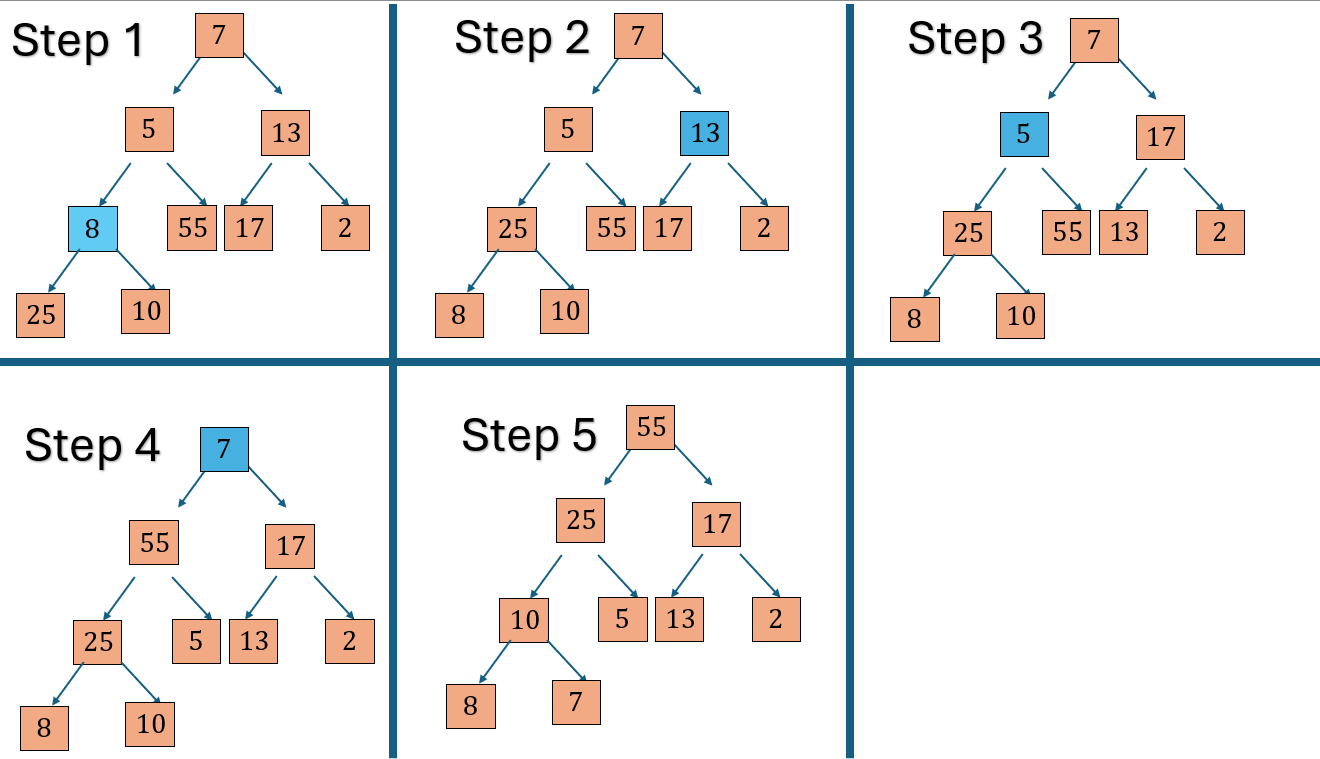
\includegraphics[width=1\textwidth]{heapBuild.png}
    
    \item Demonstrate HeapSort on the Array A:
    \subitem 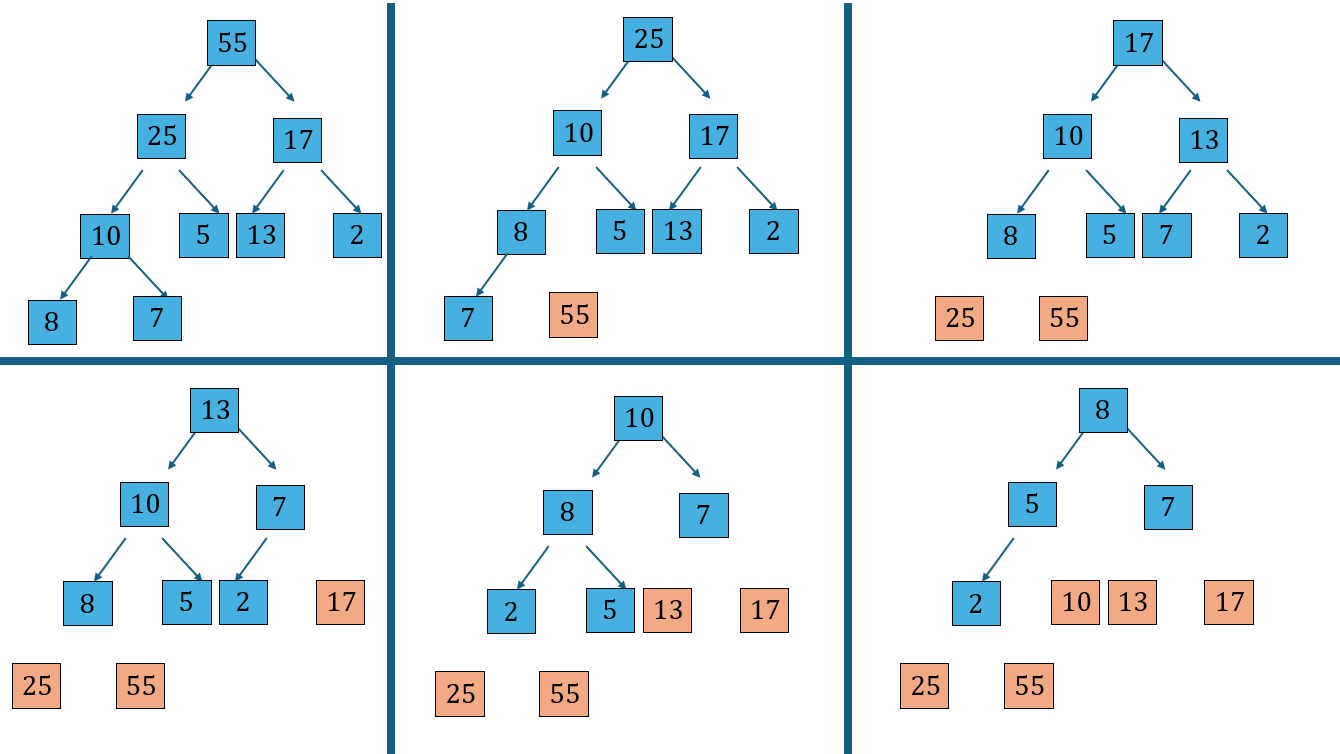
\includegraphics[width=1\textwidth]{heapSortOne.png}
    \subitem 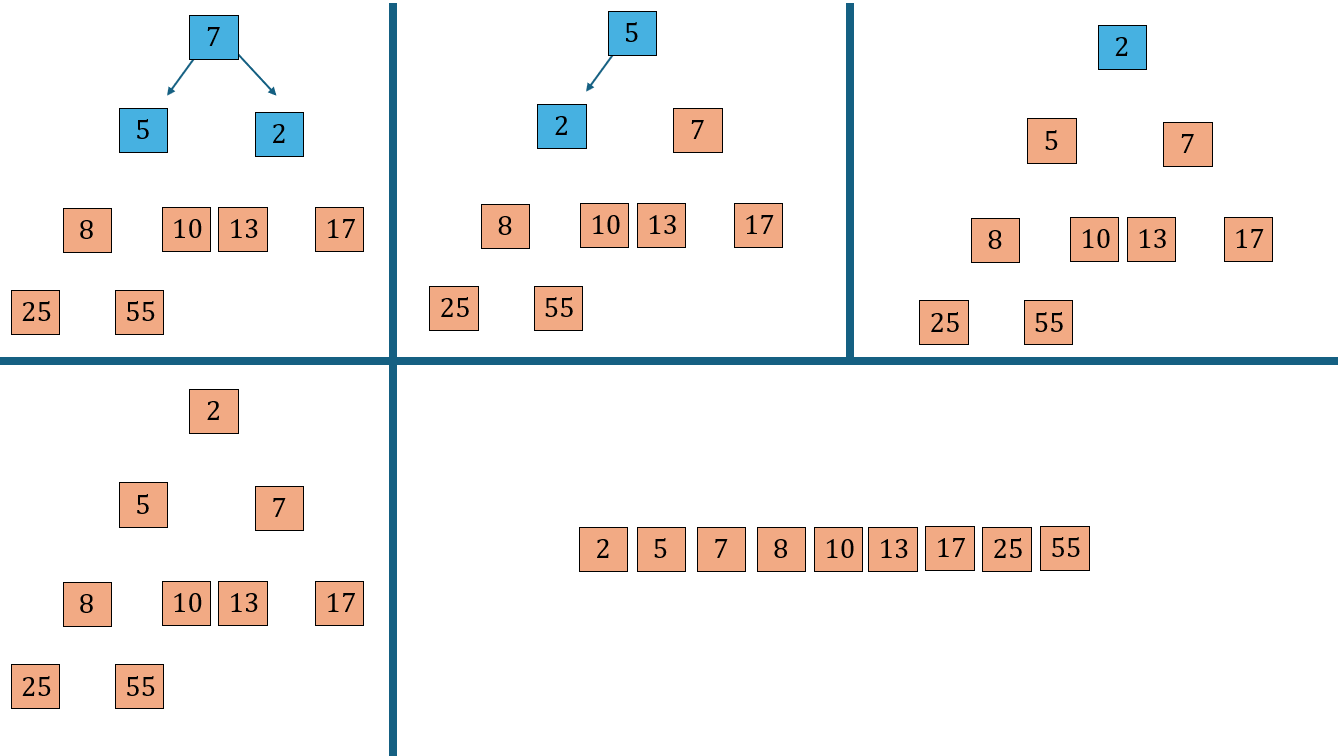
\includegraphics[width=1\textwidth]{heapSortTwo.png}
\end{enumerate}

% Question 10
\subsection*{Q10}
\begin{enumerate}[label=(\alph*)]
    \item Assume you have k sorted lists and total n items and you want to merge into 1 sorted list. Psuedocode and use a heap.
    \item Answer Description: I would first build a heap using the lists, and then call heap sort on the heap.
    \begin{lstlisting}[frame=single]
    def mergeLists(Array A):
        
        A_count = 1
        A.heap-size = n
        // Assign the values of the lists to an array
        for i = 1 to k:
            for j = 1 to list_i.Length:
                A[A_count] = lists[i][j]
                A_count = A_count + 1
    
        // Make the array into a heap
        for i = floor(n/2) to 1:
            MAX-HEAPIFY(A,i)
        
        // Sort the Array with heapsort
        for i = n to 2:
            swap A[1] with A[i]
            A.heap-size = A.heap-size - 1
            MAX-HEAPIFY(A,1)

    \end{lstlisting}
    \item I believe the time complexity to complete with algorithm will be O(n) for building the array, O(n) for making the array a heap, then sorting alone takes nlog(n). So total time complexity is n+n+nlogn or O(nlogn).


\end{enumerate}

% Question 11 (Graduate students only)
\subsection*{Q1 (Graduate students only)}
\begin{enumerate}[label=(\alph*)]
    \item Use the definition of $\omega$ and Sterlings approximation given in the book to prove that $n!$ = $\omega(2n)$.
    \subitem (1) Stirling's Approximation: $n! = \sqrt[2]{2 \pi n} * (\frac{n}{e})^n*e^{a_{n}}$
    \subitem (2) For $\omega$, we need to show $\lim_{n\to\infty} \frac{n!}{2^n} = \infty$
    \subitem (3)  $\lim_{n\to\infty} \frac{n!}{2^n} = \lim_{n\to\infty} \frac{\sqrt{2 \pi n} * (\frac{n}{e})^n*e^{a_{n}}}{2^n}$
    \subitem (4) $e^{a_{n}}$ goes to 1 as $\frac{1}{12n+1} < a < \frac{1}{12n}$. As n approaches $\infty$, $\frac{1}{12n}$ goes to 0 and $e^0 = 1$.
    \subitem (5) So we're left with: $\lim_{n\to\infty} \frac{\sqrt{2 \pi n} * (\frac{n}{e})^n}{2^n}$
    \subitem (6) $\lim_{n\to\infty} \frac{\sqrt{2 \pi n} * (\frac{n}{e})^n}{2^n}$ = $\lim_{n\to\infty} \sqrt{2 \pi n} * (\frac{n}{2e})^n$
    \subitem (7) $\sqrt{2 \pi n}$ goes to $\infty$ as n goes to $\infty$.
    \subitem (8) So, the final term to evaluation is $(\frac{n}{2e})^n$. 2e is a constant, so $\frac{n}{2e}$ is greater than one when n is sufficiently large (over about 5).
    \subitem (9) This means, $\frac{n}{2e}$ approaches $\infty$ as well!
    \subitem (10) Thus, $\lim_{n\to\infty} \frac{n!}{2^n} = \infty*\infty*1 = \infty$.
    \subitem (11) $n!$ = $\omega(2n)$. \textbf{Proof complete.}


\end{enumerate}

% Question 12 (Graduate students only)
\subsection*{Q2 (Graduate students only)}
\begin{enumerate}[label=(\alph*)]
    \item Let $T(n) = aT(n/b) + f(n)$. Prove that if f(n) is a polynomial and $f(n) = \Omega(n^{log_{b}(a+e)})$ where e>0, then Master's Theorem applies for all $a \geq 1$ and $b \geq 1$
    \subitem (1) Assumption: $f(n) \geq c * n^{log_{b}(a+e)}$
    \subitem (2) Assumption: $a \geq 1$ and $b \geq 1$
    \subitem (3) Assumption: f(n) is asymptotically positive and a polynomial.
    \subitem (4) Unfortunately need to give up on this problem. I'm going to attempt to talk it out, but I can't say I know how this works. I believe that, regardless of the values of a or b, we can show that all 3 cases of the Master Theorem work and properly bound T(n). I have attached a picture that I attempted to create for some explanation using a recurrence tree, but I don't think that is what you're looking for.
    \subitem \subitem 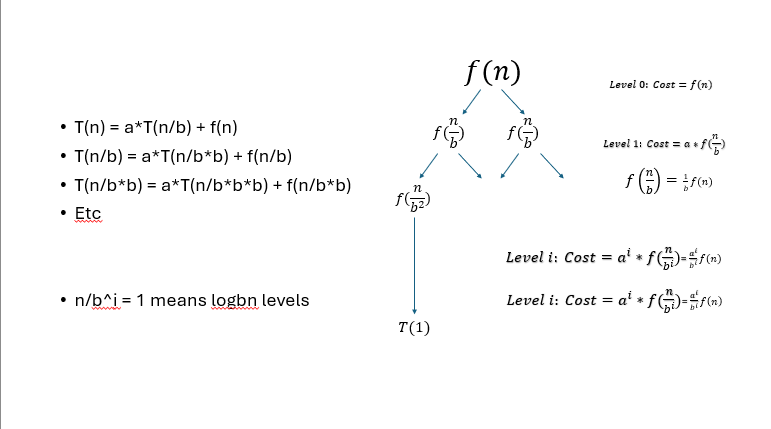
\includegraphics[width=1\textwidth]{masters.png}

\end{enumerate}

\end{document}
